% XeLaTeX document
\documentclass[12pt,a4paper]{article}

% Редактируем: конфигурация, личные настройки: имя, название предмета и пр. для титульной страницы и метаданных документа здесь
\newcommand{\university}{Национальный исследовательский Университет ИТМО}
\newcommand{\mfaculty}{Мегафакультет информационных и трансляционных технологий}
\newcommand{\faculty}{Факультет инфокоммуникационных технологий}
\newcommand{\city}{Санкт-Петербург}
\newcommand{\num}{ №4a}
\newcommand{\docname}{Типовая работа}
\newcommand{\subject}{Математика}
\newcommand{\tutorname}{С.А. Александрова}
\newcommand{\studentname}{В.Д. Козлов}
\newcommand{\group}{K3120}

% Не редактируем: используемые пакеты
% настройка кодировки, шрифтов и русского языка
\usepackage{fontspec}
\usepackage{polyglossia}

% рабочие ссылки в документе
\usepackage{hyperref}

% графика
\usepackage{graphicx}
\usepackage{tikz}

% поворот страницы
\usepackage{pdflscape}

% качественные листинги кода
\usepackage{minted}
\usepackage{listings}
\usepackage{lstfiracode}

% отключение копирования номеров строк из листинга, работает не во всех просмотрщиках (в Adobe Reader работает)
\usepackage{accsupp}
\newcommand\emptyaccsupp[1]{\BeginAccSupp{ActualText={}}#1\EndAccSupp{}}
\let\theHFancyVerbLine\theFancyVerbLine
\def\theFancyVerbLine{\rmfamily\tiny\emptyaccsupp{\arabic{FancyVerbLine}}}

% библиография
\bibliographystyle{templates/gost-numeric.bbx}
\usepackage{csquotes}
\usepackage[parentracker=true,backend=biber,hyperref=true,bibencoding=utf8,style=numeric-comp,language=auto,autolang=other,citestyle=gost-numeric,defernumbers=true,bibstyle=gost-numeric,sorting=ntvy]{biblatex}

% установка полей
\usepackage{geometry}

% нумерация картинок по секциям
\usepackage{chngcntr}

% дополнительные команды для таблиц
\usepackage{booktabs}

% для заголовков
\usepackage{caption}
\usepackage{titlesec}
\usepackage[dotinlabels]{titletoc}

% разное для математики
\usepackage{amsmath, amsfonts, amssymb, amsthm, mathtools}

% водяной знак на документе, см. main.tex
\usepackage[printwatermark]{xwatermark}

% Не редактируем: параметры используемых пакетов и не только
% настройки polyglossia
\setdefaultlanguage{russian}
\setotherlanguage{english}

% локализация
\addto\captionsrussian{
	\renewcommand{\figurename}{Рисунок}%
	\renewcommand{\partname}{Глава}
	\renewcommand{\contentsname}{\centerline{Содержание}}
	\renewcommand{\listingscaption}{Листинг}
}

% основной шрифт документа
\setmainfont{CMU Serif}
\newfontfamily\cyrillicfont{CMU Serif}[Script=Cyrillic]

% перечень использованных источников
\addbibresource{refs.bib}

% настройка полей
\geometry{top=2cm}
\geometry{bottom=2cm}
\geometry{left=2cm}
\geometry{right=2cm}
\geometry{bindingoffset=0cm}

% настройка ссылок и метаданных документа
\hypersetup{unicode=true,colorlinks=true,linkcolor=red,citecolor=green,filecolor=magenta,urlcolor=cyan,
	pdftitle={\docname},
	pdfauthor={\studentname},
	pdfsubject={\subject},
	pdfcreator={\studentname},
	pdfproducer={Overleaf},
	pdfkeywords={\subject}
}

% настройка подсветки кода и окружения для листингов
\usemintedstyle{colorful}
\newenvironment{code}{\captionsetup{type=listing}}{}

% шрифт для листингов с лигатурами
\setmonofont{FiraCode-Regular.otf}[
	SizeFeatures={Size=10},
	Path = templates/,
	Contextuals=Alternate
]

% оформления подписи рисунка
\captionsetup[figure]{labelsep = period}

% подпись таблицы
\DeclareCaptionFormat{hfillstart}{\hfill#1#2#3\par}
\captionsetup[table]{format=hfillstart,labelsep=newline,justification=centering,skip=-10pt,textfont=bf}

% путь к каталогу с рисунками
\graphicspath{{fig/}}

% Внесение titlepage в учёт счётчика страниц
\makeatletter
\renewenvironment{titlepage} {
	\thispagestyle{empty}
}
\makeatother

\counterwithin{figure}{section}
\counterwithin{table}{section}

\titlelabel{\thetitle.\quad}

% для удобного конспектирования математики
\mathtoolsset{showonlyrefs=true}
\theoremstyle{plain}
\newtheorem{theorem}{Теорема}[section]
\newtheorem{proposition}[theorem]{Утверждение}
\theoremstyle{definition}
\newtheorem{corollary}{Следствие}[theorem]
\newtheorem{problem}{Задача}[section]
\theoremstyle{remark}
\newtheorem*{nonum}{Решение}

% настоящее матожидание
\newcommand{\MExpect}{\mathsf{M}}

% объявили оператор!
\DeclareMathOperator{\sgn}{\mathop{sgn}}

% перенос знаков в формулах (по Львовскому)
\newcommand*{\hm}[1]{#1\nobreak\discretionary{} {\hbox{$\mathsurround=0pt #1$}}{}}


% водяной знак для обозначения статуса документа
%\newwatermark[allpages,color=red!5,angle=45,scale=3,xpos=0,ypos=0]{DRAFT}
\begin{document}
% Не редактируем: Титульная страница (формируется автоматически из заданной конфигурации)
\begin{titlepage}	% начало титульной страницы

	\begin{center}		% выравнивание по центру

		\large \university \\
		\large \mfaculty \\
		\large \faculty \\[6cm]
		% название института, затем отступ 6см

		\huge \subject \\[0.5cm] % название работы, затем отступ 0,5см
		\large \docname  \num \\[5.1cm]
		 %\large Разработка методов обучения с подкреплением\\[5cm]

	\end{center}


	\begin{flushright} % выравнивание по правому краю
		\begin{minipage}{0.25\textwidth} % врезка в половину ширины текста
			\begin{flushleft} % выровнять её содержимое по левому краю

				\large\textbf{Работу выполнил:}\\
				\large \studentname \\
				\large {Группа:} \group \\

				\large \textbf{Преподаватель:}\\
				\large \tutorname

			\end{flushleft}
		\end{minipage}
	\end{flushright}

	\vfill % заполнить всё доступное ниже пространство

	\begin{center}
		\large \city \\
		\large \the\year % вывести дату
	\end{center} % закончить выравнивание по центру

\end{titlepage} % конец титульной страницы

\vfill % заполнить всё доступное ниже пространство


% Не редактируем: Страница содержания (формируется автоматически из section, subsection и пр., указанных в content.tex)
% Содержание
\tableofcontents
\newpage



% Редактируем: всё остальное: вступление, др. этапы, заключение, приложение


\section{Дано}
   Проанализировать функцию 

\begin{equation}
    \centering
    \label{eq:eq1}
    y=\frac{5x}{4-x^2}
\end{equation}


\section{Решение}

\subsection{Область определения} 
    Ф-ция определена при x $\in \mathbb{R} \setminus\{-2; 2\}$
\subsection{Тип функции}\label{sec:2.2}
    Ф-ция не явяляется переодической.
    Проверим ф-цию на четность четность/нечетность:
   $ f(-x)=\frac{-5x}{4-x^2}  \Rightarrow (f(-x) \neq f(x)) \cap (f(-x) = -f(x)) \Rightarrow $ ф-ция является нечетной
\subsection{Рост функции}
    \[f’ = \frac{(5x)'(4-x^2)-5x(4-x^2)'}{(4-x^2)^2}
          = \frac{(5(4-x^2)-5x(-2x)}{(4-x^2)^2} 
          = \frac{20-5x^2+10x^2}{(4-x^2)^2} 
          = \frac{5(x^2+4)}{(4-x^2)^2}
     \]
    Таким образом, 
    \begin{equation}
    \centering
    \label{eq:eq2}
        f’ = \frac{5(x^2+4)}{(4-x^2)^2}
    \end{equation}

    График Данной функции будет выглядеть следющим образом \cite{matplotlib}
    \begin{figure}[H]
        \centering
        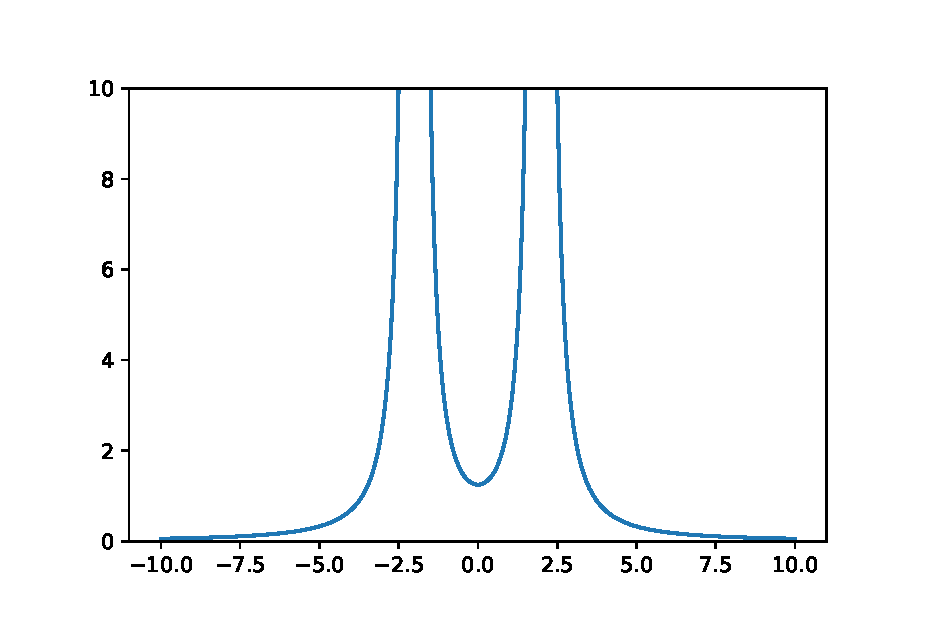
\includegraphics[height=10cm, width=15cm]{fig/firstDer.eps}
        \caption{График производной}
        \label{pic:derivative}
    \end{figure}
    Как видно из рис.~\ref{pic:derivative}, так и из самой функции производной можно с легкостью сделать вывод, что фунция возрастает на всей области определения
    
    

    
    
\subsection{Выпуклость функции}
    Возьмем вторую производную, чтобы узнать промежутки, в которых ф-ция выпукла вверх/вниз
    \begin{equation*}
        y'' = \frac{5((x^2+4)'(4-x^2)^2-(x^2+4)((4-x^2)^2)')}{(4-x^2)^4} =
        \frac{10x(x^2+12)}{4-x^2}
    \end{equation*}
    
    \begin{equation}
        \centering
        \label{eq:eq3}
        y'' =  \frac{10x(x^2+12)}{4-x^2}
    \end{equation}
    
    График данной функции будет выглядеть следющим образом \cite{matplotlib}
    \begin{figure}[H]
        \centering
        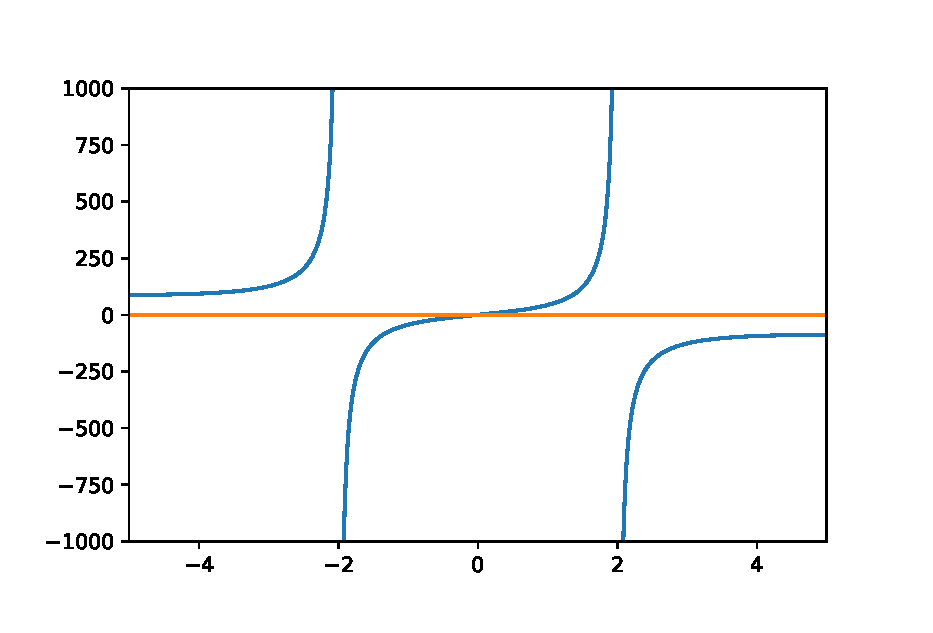
\includegraphics[width=\textwidth]{fig/secDer.eps} 
        \caption{График второй производной}
        \label{fig:my_label}
    \end{figure}
    Из этого можно сделать вывод, что ф-ция выпукла вверх при \\ $x \in (-\infty;-2)\cup(2;+\infty)$, а вниз во всех остальных точках определения ф-ции
    
\subsection{Нахождение асимптот}
    \subsubsection{Вертикальные асимптоты}
        Т.к. ф-ция не определена при $x = \pm2$, то целесообразно проверить эти точки на наличиеа асимптот:
        
        \noindent\begin{minipage}{.5\linewidth}
        \begin{equation}
            \label{eq:eq4}
            \lim_{x \to 2-0} \frac{5x}{4-x^2}=+\infty
        \end{equation}
        \end{minipage}%
        \begin{minipage}{.5\linewidth}
        \begin{equation}
            \label{eq:eq5}
            \lim_{x \to 2+0} \frac{5x}{4-x^2}=-\infty
        \end{equation}
        \end{minipage}
        
         Из $\eqref{eq:eq4}$ и  $\eqref{eq:eq5}$ следует, что $x = 2$ - вертикальная асимптота.\cite{zorichMath}
            
        \noindent\begin{minipage}{.5\linewidth}
        \begin{equation}
            \label{eq:eq6}
            \lim_{x \to -2-0} \frac{5x}{4-x^2}=+\infty
        \end{equation}
        \end{minipage}
        \begin{minipage}{.5\linewidth}
        \begin{equation}
            \label{eq:eq7}
            \lim_{x \to -2+0} \frac{5x}{4-x^2}=-\infty
        \end{equation}
        \end{minipage}
        \noindent Из $\eqref{eq:eq6}$ и  $\eqref{eq:eq7}$ следует, что $x = -2$ - вертикальная асимптота.
    \subsubsection{Горизонтальные асимптоты}
        Проверим существованиt(найдем) горизонатальные асимптоты:
        \begin{equation}
            \centering
            \label{eq:eq7}
            \lim_{x \to \infty} \frac{5x}{4-x^2}= \frac{5}{\infty} = 0
        \end{equation}
        \noindent Из $\eqref{eq:eq7}$ следует, что y=0 - горизонатальная асимптота
\subsection{Найдем точки пересечения ф-ции с координатными осями}
    \noindent\begin{minipage}{.5\linewidth}
        \begin{equation*}
            Ox:\frac{5x}{4-x^2}=0 \Rightarrow x=0
        \end{equation*}
        \end{minipage}%
        \begin{minipage}{.5\linewidth}
        \begin{equation*}
            Oy: y(0)=0 
        \end{equation*}
        \end{minipage}
\subsection{Найдем дополнительные точки}
	\begin{center}
		\begin{tabular}{|l|c|c|c|c|}
			\hline
			X & 1 & 1.5 & 3 & 5 \\ \hline
			Y & $\frac{5}{3}$ & $\frac{30}{7}$ & -3 & -$\frac{25}{21}$\\ \hline
		\end{tabular}
		\label{tabular:tab}
	\end{center}
	Нам этих точек хватит, так как ф-ция нечетная, что мы выяснили в секции \ref{sec:2.2}
	
\subsection{Начертим график}
    \begin{figure}[H]
        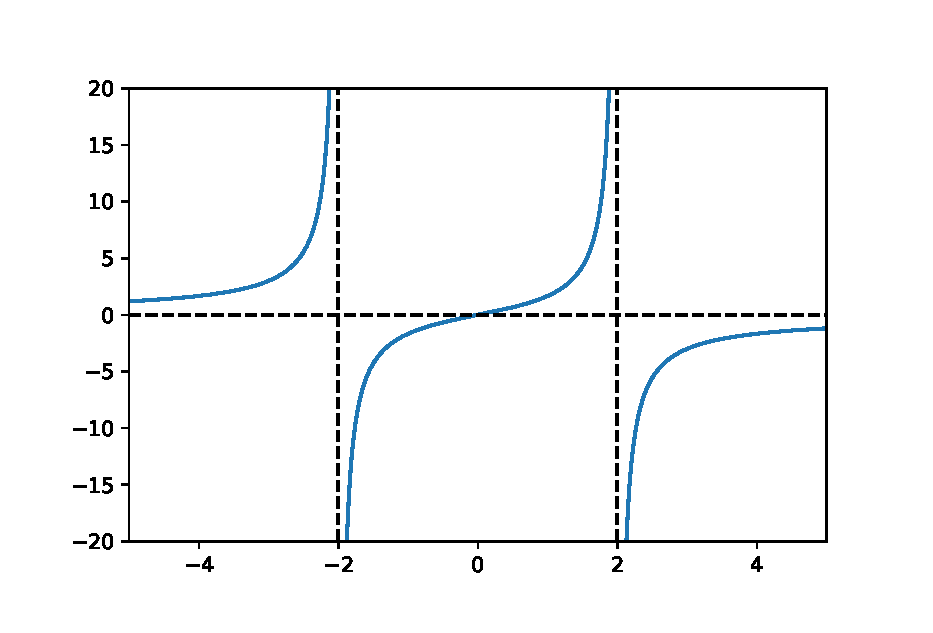
\includegraphics[width=\textwidth]{fig/mainPlot.eps} 
        \caption{график для $\eqref{eq:eq1}$}
        \label{fig:mainPlot}
    \end{figure}
    
\newpage
\section{Листинг}
    Это код, который был использован для создания рис. ~\ref{fig:mainPlot}
    \begin{code}
    	\inputminted[breaklines=true, xleftmargin=1em, linenos, frame=single, framesep=10pt, fontsize=\footnotesize, firstline=1, lastline=33]{python}{listings/python_code.py}
    	\caption{Питон - в массы)))}
    \end{code}

\newpage
\section*{Заключение}
В ходе проделанной типовой работы я смог проанализировать поведение ф-ции и построить её график, используя matplotlib
\addcontentsline{toc}{section}{Заключение}

% Не редактируем: Страница библиографии (формируется автоматически из книжек, указанных в refs.bib и пометок \cite{имя_источника} в тексте)
\newpage
\printbibliography[title=Список использованных источников]
\addcontentsline{toc}{section}{Список использованных источников}
\end{document}
